\section{Aufgabe 2} \label{ex2}

Konfiguration des IP Cores zur Realisierung der Kommunikation zwischen Prozessor und 
Peripherie als Blockdesign in Vivado 2016.2. Eingebunden in diese wurden zusätzlich die 8Bit-LED-Anzeige und anschließend der Aufbau in VHDL synthetisiert.

\subsection{Beschreibung der Funktion XGpio\_DiscreteWrite}
3 Checks ob Pointer valide, Status Ready, welcher Channel aktiv ist und ob zwei Kanäle von der Hardware unterstützt werden. Danach werden Basispointer und Adressoffset addiert und an XGPio\_WriteReg übergeben. Kanäle (Registerbänke) liegen im Speicher nacheinander, ein Umschalten erfolgt über einen Adressoffset.\\

\subsection{Woran/Wo sieht man die Antwort von der Vorbereitung im Code?}
In der Funktion XGPIO\_Initialize wird über die DeviceID ein Instanz-Zeiger (InstancePtr) erzeugt und initalisiert. Dieser Instanz-Zeiger wird später verwendet, um die genaue Adresse zu berechnen. Die Offsets können zum konfigurieren der I/Os als (Ein- oder Ausgang) und zum setzen der einzelnen Bits verwenden werden.\\

\begin{minipage}{\textwidth}
    \begin{center}        
        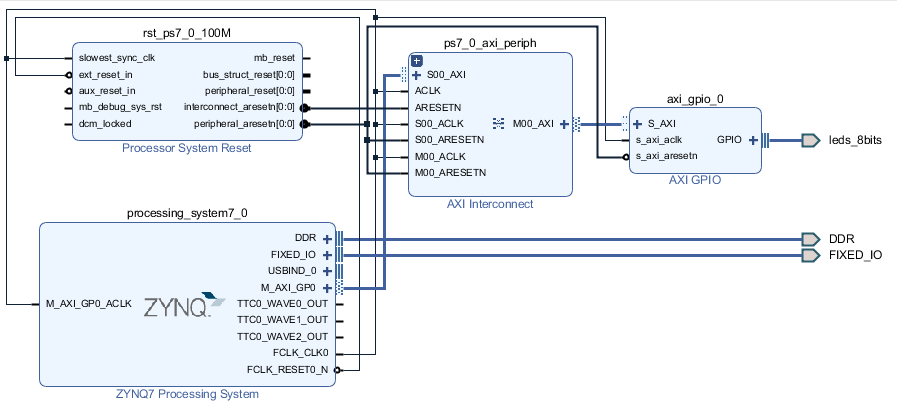
\includegraphics[scale=0.7]{img/a2.png} 
    \end{center}
\end{minipage}
\begin{center}
Vivado: Schemaplan der IP-Cores
\end{center}


